\section{Recombination Metaheuristics}

Constructive and exchange heuristics manage one solution at a time (except for the Ant System).\\

Recombination heuristics \textbf{manage several solutions in parallel}
\begin{itemize}
	\item \textbf{Start from a set} (population) \textbf{of solutions} (individuals) obtained somehow.\\
	
	\item \textbf{Recombine the individuals} generating a new population.\\
\end{itemize}

Their original aspect is the \textbf{use of operations working on several solutions}, but they often include features of other approaches (sometimes renamed).\\

Some are nearly or fully deterministic
\begin{itemize}
	\item Scatter Search
	\item Path Relinking
\end{itemize}

others are strongly randomized (often based on biological metaphors)
\begin{itemize}
	\item genetic algorithms
	\item memetic algorithms
	\item evolution strategies
\end{itemize}

Of course the effectiveness of a method does not depend on the metaphor.\\

\newpage

\paragraph{General scheme:} The \textbf{basic idea} is that
\begin{itemize}
	\item \textbf{Good solutions share components} (anything that forms the solution) with the \textbf{global optimum}.\\
	
	\item \textbf{Different solutions} can \textbf{share different components}.\\
	
	\item \textbf{Combining different solutions}, it is possible to \textbf{merge optimal components} more easily than building them step by step.\\
\end{itemize}

The typical scheme of recombination heuristics is
\begin{itemize}
	\item Build a \textbf{starting population of solutions} (generated in any way).\\
	
	\item As long as a suitable \textbf{termination condition does not hold}.\\
	
	\item At \textbf{each iteration} (usually called "generation" to distinguish it from more basic concepts of iteration) \textbf{update the population}
	\begin{itemize}
		\item \textbf{extract single individuals} and \textbf{apply exchange operations} to them
		\item \textbf{extract subsets of individuals} (usually, pairs) and \textbf{apply recombination operations} to them
		\item \textbf{collect the individuals} thus generated and \textbf{choose whether to accept or not} each of them and how many copies \textbf{into the new population}
	\end{itemize}
	
\end{itemize}

\newpage

\subsection{Scatter Search}

Scatter Search (SS), proposed by Glover (1977), proceeds as follows
\begin{enumerate}
	\item \textbf{Generate} a \textbf{starting population} of solutions.\\
	
	\item \textbf{Improve all of them} with an \textbf{exchange procedure}.\\
	
	\item build a \textbf{reference set} $R = B \cup D$ where
	\begin{itemize}
		\item \textbf{subset} $B$ includes the \textbf{best known solutions}
		\item \textbf{subset} $D$ includes the \textbf{"farthest" solutions} from $B$ and each other (this requires a distance definition, e.g., the Hamming distance)
	\end{itemize}
	\nn
	
	\item For \textbf{each pair of solutions} $(x, y ) \in B \times (B \cup D)$
	\begin{itemize}
		\item "\textbf{recombine}" $x$ and $y$, \textbf{generating} $z$
		
		\item \textbf{improve} $z$ \textbf{obtaining} $z'$ with an \textbf{exchange procedure}
		
		\item if $z' \notin B$ and $B$ contains a \textbf{worse solution}, \textbf{replace it} with $z'$ (we want no duplicates in the reference set); i.e., if it's better than any solution in our set of best solutions replace it.
		
		\item if $z' \notin D$ and $D$ includes a \textbf{closer solution}, \textbf{replace it} with $z'$ (we want no duplicates in the reference set); i.e., if it's further away than any solution in our set of farthest solutions replace it.
	\end{itemize}
	\nn
	
	\item Terminate when $R$ is unchanged.\\
\end{enumerate}

The rationale is that
\begin{itemize}
	\item the \textbf{recombinations in} $B \times B$ \textbf{intensify} the search
	
	\item the \textbf{recombinations in} $B \times D$ \textbf{diversify} the search
\end{itemize}

\newpage

\begin{algorithm}[H]
	\caption{Algorithm $ScatterSearch(I , P, n_B , n_D)$}
	\begin{algorithmic}
		\STATE $B := \emptyset$ 
		\STATE $D := \emptyset$
		\REPEAT
		\STATE $Stop = true$
		\FOR{each $x \in P$}
		\STATE $z := SteepestDescent(I , x)$
		\IF{$f (z) < f (x^\ast)$}
		\STATE $x^\ast := z$
		\ENDIF
		\STATE $y_B := \arg \max_{y \in B} \, f(y)$
		\STATE $y_D := \arg \min_{y \in D} \, d (y , B \cup D \setminus \{y \})$
		\IF{$z \notin B$ and ($|B| < n_B$ or $f (z) < f (y_B )$)}
		\STATE // $B$ keeps the $n_B$ best unique solutions
		\STATE $B := B \cup \{z\}$
		\STATE $Stop := false$ 
		\IF{$|B| > n_B$} 
		\STATE $B := B \setminus \{y_B \}$
		\ENDIF
		\ELSE 
		\IF{$z \notin D$ and ($|D| < n_D$ or $d (z, B \cup D \setminus \{y_D \}) > d (y_D , B \cup D \setminus \{y_D \})$)}
		\STATE // $D$ keeps the $n_D$ most diverse unique solutions
		\STATE $D := D \cup \{z\}$ 
		\STATE $Stop := false$ 
		\IF{$|D| > n_D$} 
		\STATE $D := D \setminus \{y_D \}$
		\ENDIF
		\ENDIF
		\ENDIF
		\ENDFOR
		\STATE $P := \emptyset$
		\FORALL{$(x, y ) \in B \times (B \cup D)$} 
		\STATE // Recombine to build the new population
		\STATE $P := P \cup Recombine(x, y , I )$
		\ENDFOR
		\UNTIL{$Stop = true$}
		\RETURN $(x^\ast, f (x^\ast))$
	\end{algorithmic}
\end{algorithm}

\newpage

\subsubsection{Recombination procedure}
The recombination procedure depends on the problem.\\

Usually, solutions $x$ and $y$ are \textbf{manipulated as subsets}
\begin{enumerate}
	\item Include in $z$ \textbf{all the elements shared by} $x$ \textbf{and} $y$:
	$$ z := x \cap y $$
	both solutions concur in suggesting those elements, it's probably good if both include it.\\
	
	\item \textbf{Augment solution} $z$ \textbf{adding elements from} $x \setminus z$ or $y \setminus z$
	\begin{itemize}
		\item chosen at random or with a greedy selection criteria
		\item alternatively from each source or freely from the two sources (this is similar to a restricted constructive heuristic)
	\end{itemize}
	add elements that are in $x$ or $y$ (and not already in $z$), it's not choosing elements from the whole ground set.\\
	
	\item If necessary, \textbf{add external elements} from $B \setminus (x \cup y)$.\\
	
	\item If subset $z$ \textbf{is unfeasible}, apply an \textbf{auxiliary exchange heuristic} to make it feasible (\textbf{repair} procedure).\\
\end{enumerate}

\newpage

\paragraph{Examples:}
\begin{itemize}
	\item \textbf{MDP}
	\begin{itemize}
		\item start with $z := x \cap y$
		\item augment $z$ with $k - |z|$ random or greedy points from $x \setminus z$ or $y \setminus z$ (add missing points taking them from the solutions)
		\item no repair procedure is required
	\end{itemize}
	\nn
	
	\item \textbf{Max-SAT}
	\begin{itemize}
		\item start with $z := x \cap y$
		\item augment $z$ with $n - |z|$ random or greedy truth assignments from $x \setminus z$ or $y \setminus z$ 
		\item no repair procedure is required
	\end{itemize}
	\nn
	
	\item \textbf{KP}
	\begin{itemize}
		\item start with $z := x \cap y$
		\item augment $z$ with random or greedy elements from $x \setminus z$ or $y \setminus z$ respecting the capacity
		\item no repair procedure is required
		\item the solution could be augmented with elements from $B \setminus (x \cup y)$ (there could still be space)
	\end{itemize}
	\nn
	
	\item \textbf{SCP}
	\begin{itemize}
		\item start with $z := x \cap y$
		\item augment $z$ with random or greedy columns from $x \setminus z$ or $y \setminus z$ (avoiding the redundant ones)
		\item remove the redundant columns with a destructive phase
	\end{itemize}
	\nn
\end{itemize}

You always start from the intersection, then "fill" the answer with elements from the first two solutions, in the end complete the solution by either augmenting or repairing it.\\

\newpage

\subsection{Path Relinking}
Path Relinking (PR), proposed by Glover (1989), is generally used as a final intensification procedure more than as a stand-alone method.\\

Given a \textbf{neighborhood} $N$ and an \textbf{exchange heuristic based on it}
\begin{itemize}
	\item Collect in a \textbf{reference set} $R$ the \textbf{best solutions} generated by the \textbf{auxiliary heuristic} (\textbf{elite solutions}).\\
	
	\item \textbf{For each pair of solutions} $x$ and $y$ in $R$
	\begin{itemize}
		\item \textbf{build a path} $\gamma_{xy}$ \textbf{from} $x$ \textbf{to} $y$ \textbf{in the search space of neighborhood} $N$ applying to $z^{(0)} = x$ the auxiliary exchange heuristic, but \textbf{choosing at each step the solution closest to the destination} $y$
		$$ z^{(k+1)} := \arg \min_{z \in N(z^{(k)})} d (z, y ) $$
		where $d$ is a suitable metric function on the solutions. In case of equal distance, optimize the objective function $f$
		
		\item \textbf{find} the \textbf{best solution} $z_{xy}^\ast$ \textbf{along the path} (and improve it)
		$$ z^\ast_{xy} := \arg \min_{k \in \{1 , \, ... \, , |\gamma_{xy}| - 1} f (z^{(k)}) $$
		
		\item if $z^\ast_{xy} \notin R$ and is \textbf{better than the worst in} $R$, \textbf{add it} to $R$
	\end{itemize}
	\nn
\end{itemize}

Basically, it takes two good solutions from a reference set and finds a (greedy) path between them, searching for an even better solution, which can be added to the reference set, if it's good enough. For every pair the best solution gets added to the population and the process repeated until the algorithm can't improve anymore.\\

\newpage

\begin{algorithm}[H]
	\caption{Algorithm $PathRelinking(I , P, n_R )$}
	\begin{algorithmic}
		\REPEAT
		\STATE $R := \emptyset$
		\FOR{each $x \in P$}
		\STATE $z := SteepestDescent(I , x)$
		\IF{$f (z) < f (x^\ast)$} 
		\STATE $x^\ast := z$
		\ENDIF
		\STATE $y_R := \arg \max_{y\in R} f (y )$
		\IF{$z \notin R$ and ($|R| < n_R$ or $f (z) < f (y_R )$)}
		\STATE // $R$ keeps the $n_R$ best unique solutions
		\STATE $R := R \cup \{z\}$ 
		\STATE $Stop := false$
		\IF{$|R| > n_R$}
		\STATE $R := R \setminus \{y_R \}$
		\ENDIF
		\ENDIF
		\ENDFOR
		\STATE $P := \emptyset$
		\FOR{each $x \in R$ and $y \in R \setminus \{x\}$} 
		\STATE // Recombine to build the new population
		\STATE $z := x$
		\STATE $z^\ast := x$
		\WHILE{$z \neq y$} 
		\STATE // Build a path from $x$ to $y$
		\STATE $Z := \arg \min_{z' \in N(z)} d (z', y )$
		\STATE $z := \arg \min_{z' \in Z} f (z')$
		\IF{$f (z) < f (z^\ast)$} 
		\STATE $z^\ast := z$
		\ENDIF
		\ENDWHILE
		\IF{$z^\ast \notin P$} 
		\STATE $P := P \cup \{z^\ast\}$
		\ENDIF
		\ENDFOR
		\UNTIL{$Stop = true$}
		\RETURN $(x^\ast, f (x^\ast))$
	\end{algorithmic}
\end{algorithm}

\newpage

The paths explored in this way
\begin{itemize}
	\item \textbf{Intensify} the search, because they \textbf{connect good solutions}.\\
	
	\item \textbf{Diversify} the search, because they \textbf{follow different paths} with respect to the exchange heuristic (especially if the extremes are far away)
\end{itemize}

Since the \textbf{distance} of $z^{(k)}$ from $y$ is \textbf{decreasing}, one can explore 
\begin{itemize}
	\item \textbf{Worsening solutions} without the risk of cyclic behaviors.\\
	
	\item \textbf{Unfeasible subsets} without the risk of not getting back to feasibility (they do not improve directly, but open the way to improvements).\\
\end{itemize}

\subsubsection{Variants}

Given two solutions $x$ and $y$, Path Relinking has several variants:
\begin{itemize}
	\item \textbf{Forward path relinking:} build a path from the worse to the better one.\\
	
	\item \textbf{Backward path relinking:} build a path from the better to the worse one.\\
	
	\item \textbf{Back-and-forward path relinking:} build both paths.\\
	
	\item \textbf{Mixed path relinking:} build a path with alternative steps from each extreme (updating the destination).\\
	
	\item \textbf{Truncated path relinking:} build only the first steps of the path (if the good solutions are experimentally close to each other).\\
	
	\item \textbf{External path relinking:} build a path from one moving away from the other (if the good solutions are experimentally far from each other).\\
\end{itemize}

% End of L21

\newpage

\subsection{Encoding-based algorithms}

Many recombination heuristics define and \textbf{manipulate encodings of the solutions} (i.e., compact representations), \textbf{rather than the solutions}.\\

The aims of this approach are
\begin{itemize}
	\item \textbf{Abstraction:} conceptually distinguishing the method from the problem to which it is applied.\\
	
	\item \textbf{Generality:} build operators effective on every problem represented with a given family of encodings. This doesn't require knowledge of the original problem.\\
\end{itemize}

In a strict sense, every representation of a solution in memory is an encoding: the term "encoding" tends to be used for the more involved and compact ones. The difference is blurred.\\

\newpage

\subsection{Genetic Algorithm}

The genetic algorithm, proposed by Holland (1975), is the most famous among the encoding algorithms, but there's a large family of similar methods.\\

It \textbf{builds and encodes a population} $X^{(0)}$, and \textbf{repeatedly applies}:
\begin{enumerate}
	\item \textbf{Selection:} generate a new population starting from the current one
	\item \textbf{Crossover:} recombine subsets of two or more individuals
	\item \textbf{Mutation:} modify the individuals (complementary to the crossover)
\end{enumerate}

\nn

\begin{algorithm}[H]
	\caption{Algorithm $GeneticAlgorithm(I , X^{(0)})$}
	\begin{algorithmic}
		\STATE $\Xi^{(0)} := Encode(X^{(0)})$
		\STATE $x^\ast := \arg \min_{x \in X^{(0)}} f(x)$ // Best solution found so far
		\FOR{$g = 1$ to $n_g$}
		\STATE $\Xi := Selection(\Xi)$
		\STATE $\Xi := Crossover(\Xi)$
		\STATE $x_c := \arg \min_{\xi \in \Xi} f (x (\xi))$
		\IF{$f (x_c) < f (x^\ast)$} 
		\STATE $x^\ast := x_c$
		\ENDIF
		\STATE $\Xi := Mutation(\Xi)$
		\STATE $x_m := \arg \min_{\xi \in \Xi} (x (\xi))$
		\IF{$f (x_m) < f (x^\ast)$} 
		\STATE $x^\ast := x_m$
		\ENDIF
		\ENDFOR
		\RETURN $(x^\ast, f (x^\ast))$
	\end{algorithmic}
\end{algorithm}

Start from a population $X^{(0)}$ (obtained in any way), encode it into $\Xi^{(0)}$, get the best solution, for each of the $n_g$ generation do selection, crossover, check the best, mutation, check the best again. In the end return the best solution found overall.\\

\newpage

\subsubsection{Features of a good encoding}
The performance of a genetic algorithm depends on the encoding.\\

The \textbf{following properties} should be \textbf{satisfied} (with decreasing importance)
\begin{enumerate}
	\item \textbf{Each solution should have an encoding}, except for dominated ones; otherwise, there would be unreachable solutions.\\
	
	\item \textbf{Different solutions} should have \textbf{different encodings} (or the best solution with a given encoding should be easy to find); otherwise, there would be unreachable solutions. \\
	
	\item \textbf{Each encoding} should correspond to a \textbf{feasible solution}; otherwise, the population would include useless individuals. This doesn't necessarily mean that there's a 1 to 1 correspondence, a single solution can have multiple encodings.\\
	
	\item \textbf{Each solution} should correspond to the \textbf{same number of encodings}; otherwise, some solutions would be unduly favored.\\
	
	\item The \textbf{encoding and decoding operations} should be \textbf{efficient}, otherwise, the algorithm would be inefficient.\\
	
	\item \textbf{Locality:} \textbf{small changes to the encoding} should induce \textbf{small changes to the solution}, otherwise intensification and diversification would be impossible.\\
\end{enumerate}

These conditions \textbf{depend very much on the constraints of the problem} (so much for abstraction...).\\

\newpage

\paragraph{Feasible and unfeasible encodings:} Mutation and crossover operators \textbf{easily produce unfeasible subsets}.\\

If property 3 is not satisfied; this may imply the \textbf{violation of}
\begin{enumerate}
	\item \textbf{Quantitative constraints} (e.g., a capacity is exceeded).\\
	
	\item \textbf{Structural constraints} (e.g., the solution is not made of circuits).\\
\end{enumerate}

The second kind of infeasibility is harder to repair, because it concerns constraints that interact more strongly with each other.\\

The encoding can lead wherever inside the $2^B$ possibilities
\begin{center}
	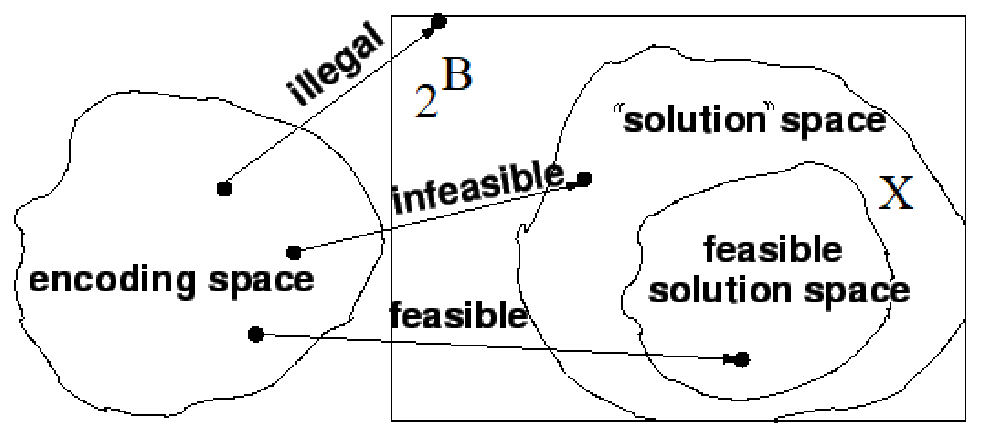
\includegraphics[width=0.75\columnwidth]{img/feasible1}
\end{center}
Often there's a feasible region, but some constraints (usually quantitative) to obtain a "solution space", with elements that are not solutions, strictly speaking, but they are kinda similar, so we call them unfeasible solutions. E.g., solutions that exceed capacity in the BPP, they will not be feasible, but they \textit{look like} a solution, structurally speaking it makes sense.\\

Some encodings \textbf{guarantee structural} (though not quantitative) \textbf{feasibility}.\\

\newpage

\subsubsection{Encodings}

\paragraph{The incidence vector:} The most direct \textbf{encoding} for Combinatorial Optimization problems is the \textbf{binary incidence vector} $\xi \in \mathbb{B}^{|B|}$
$$ 
\begin{cases}
	\xi_i = 1 & \text{ indicates that } i \in x \\
	\xi_i = 0 & \text{ indicates that } i \notin x
\end{cases}
$$

A generic binary vector \textbf{corresponds}
\begin{itemize}
	\item In the \textbf{KP} to a \textbf{set of objects}: its weight could be excessive.\\
	
	\item In the \textbf{SCP} to a \textbf{set of columns}: it could leave uncovered rows.\\
	
	\item In the \textbf{PMSP} and in the \textbf{BPP} to a \textbf{set of assignments of tasks} (objects) \textbf{to machines} (containers): it could make zero or more assignments for an element; in the BPP, it could violate the capacity of some containers.\\
	
	\item In the \textbf{TSP} to a \textbf{set of arcs}: it could not form a Hamiltonian circuit.\\
	
	\item In the \textbf{CMSTP} (\textbf{VRP}) to a \textbf{set of edges} (\textbf{arcs}): it could not form a tree (set of cycles), or exceed the capacity of the subtrees (circuits).\\
\end{itemize}

Basically, if $0$ the element is not in the solution, if $1$ it is.\\

\newpage

\paragraph{Symbolic strings:} If the \textbf{ground set} is \textbf{partitioned into components} (objects, tasks, Boolean variables, vertices, nodes...)
$$ B = \bigcup_{c \in C} B_c \;\;\; \text{ with } B_c \cap B_{c'} = \emptyset \text{ for each } c \neq c' $$

and the \textbf{feasible solutions contain one element of each component}
$$ |x \cap B_c| = 1 \text{ for each } c$$

Example: the assignment of each variable in the Max-SAT problem is a component each, the solution consists of a single value for each of these components (each variable assignment).\\

One can
\begin{itemize}
	\item \textbf{Define for each} $c \in C$ \textbf{an alphabet} of symbols \textbf{describing component} $B_c$.\\
	
	\item \textbf{Encode the solution into a string of symbols} $\xi \in B_1 \times \, ... \, \times B_{|C |}$
	$$ \xi_c = \alpha \text{ indicates that } x \cap B_c = \{(c, \alpha)\} $$ 
	this means that component $c$ is assigned to $\alpha$.\\
\end{itemize}

Define an alphabet for the values of each component and thus the solutions can be described by a sequence of symbols, one for each component. Example, for the BPP by putting in sequence the "names" of the container the first symbol is the assignment of the first object, the second symbol is the assignment of the second object and so on.\\

\newpage

Examples of encodings:
\begin{itemize}
	\item \textbf{Max-SAT:} a string of $n$ Boolean values, one for each logical variable.\\
	
	\item \textbf{PMSP:} a string of machine labels, one for each task.\\
	
	\item \textbf{BPP/CMSTP:} a string of container/subtree labels, one for each object/vertex:
	\begin{itemize}
		\item the structural constraint on object assignment is enforced
		\item the quantitative constraint on capacity is neglected
	\end{itemize}
	\nn
	
	\item For the \textbf{VRP}, a string of vehicle labels, one for each node (but capacity is neglected and decoding the circuit for each vehicle is an $\mathcal{NP}$-complete problem).\\
	
	\item The solutions of the \textbf{TSP}, the \textbf{KP}, the \textbf{SCP} are \textbf{not partitions}.\\
\end{itemize}

\newpage

\paragraph{Permutations of a set:} A common encoding is given by the \textbf{permutations of a set}
\begin{itemize}
	\item If the \textbf{solutions are permutations}, this is the \textbf{natural encoding} (TSP solutions are subsets of arcs, but also permutations of nodes).\\
	
	\item If the \textbf{solutions are partitions} and the \textbf{objective is additive on} the subsets, the \textbf{order-first split-second method transforms permutations into partitions} (but solutions and encodings do not correspond one-to-one!).\\
	
	\item If the problem \textbf{admits a constructive algorithm that at each step}
	\begin{enumerate}
		\item chooses an element
		\item chooses how to add it to the solution (if many ways exist)
	\end{enumerate}
	we can \textbf{feed elements to the algorithm following the permutation} (if step 2 is not unique, some solutions could have no encoding)
\end{itemize}

\newpage

\subsubsection{Selection}

At \textbf{each generation} $g$ a \textbf{new population} $\Xi^{(g)}$ is built \textbf{extracting} $n_p = |\Xi^{(g )}|$ \textbf{individuals from the current population} $\Xi^{(g-1)}$ (typically they have the same cardinality)
$$ \Xi^{(g )} := Selection(\Xi^{(g −1)}) $$

The \textbf{extraction} follows \textbf{two fundamental criteria}
\begin{enumerate}
	\item \textbf{An individual can be extracted more than once}.\\
	
	\item \textbf{Better individuals are extracted with higher probability}
	$$ \varphi (\xi) > \varphi (\xi') \implies \pi_{\xi} \geq \pi_{\xi'} $$
	where the \textbf{fitness} $\varphi (\xi)$ is a \textbf{measure of the quality of individual} $\xi$
	\begin{itemize}
		\item for a maximization problem, commonly
		$$ \varphi (\xi) = f (x(\xi)) $$
		(simply the objective function)
		
		\item for a minimization problem, commonly
		$$ \varphi (\xi) = UB - f (x (\xi)) $$
		where $UB \geq f^\ast$ is a suitable upper bound on the optimum (this is to have a higher fitness for higher quality of individual)
	\end{itemize}
\end{enumerate}

We need to transform fitness into probability, but how? \\

\newpage

\paragraph{Proportional selection:} The original scheme proposed by Holland (1975) assumed a \textbf{probability proportional to fitness}
$$ \pi_{\xi} = \frac{\varphi (\xi)}{\sum_{\xi \in \Xi} \varphi (\xi)} $$

This is named \textbf{roulette-wheel selection} or \textbf{spinning wheel selection:}
\begin{itemize}
	\item given the \textbf{fitness for} $\xi_i \in \Xi (i = 1, \, ... \, , n_p )$
	
	\item \textbf{build the intervals} 
	$$ \Gamma_i = \left( \sum_{k=1}^{i-1} \pi_{\xi_i}; \, \sum_{k=1}^{i} \pi_{\xi_i} \right] $$
	in $O (n_p )$ time
	
	\item \textbf{extract a random number} $r \in U (0; 1]$
	
	\item \textbf{choose individual} $i^\ast$ \textbf{such that} $r \in \Gamma_{i^\ast}$ in $O (\log n_p )$ time each
\end{itemize}

\begin{center}
	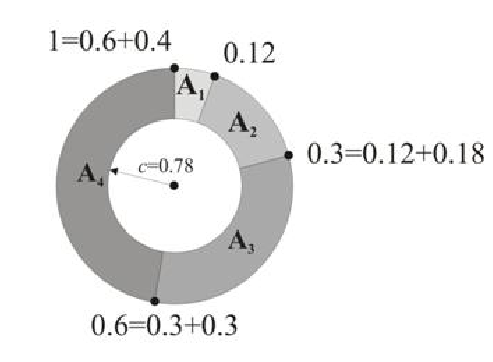
\includegraphics[width=0.5\columnwidth]{img/selectionwheel}
\end{center}

You compute all fitness values, normalize it from $0$ to $1$, assign a segment of $(0; 1]$ to every element. Extract a random value from $0$ to $1$ which will correspond to a segment and thus an element.\\

Overall $O (n_p \log n_p)$ time.\\

\newpage


The \textbf{proportional selection suffers from}
\begin{itemize}
	\item \textbf{stagnation:} in the long term, all individuals tend to have a good fitness, and therefore similar selection probabilities
	\item \textbf{premature convergence:} if the best individuals are bad and the other ones very bad, the selection quickly generates a bad population
\end{itemize}

\nn

\paragraph{Rank selection:} To overcome these limitations, one should \textbf{at the same time}
\begin{itemize}
	\item assign \textbf{different probabilities to the individuals}
	\item \textbf{limit} the \textbf{difference of probability among the individuals}
\end{itemize}

The \textbf{rank selection method}
\begin{itemize}
	\item \textbf{sorts the individuals by non-decreasing fitness}
	$$ \Xi^{(g )} = \{ \xi_1, \, ... \, , \xi_{np}\} \text{ with } \varphi_{\xi_1} \leq \, ... \, \leq \varphi_{\xi_{np}} $$
	
	\item \textbf{assigns to the} $k$-th individual a \textbf{probability equal to}
	$$ \pi_{\xi_k} = \frac{k}{\sum_{k=1}^{n_p} k} = \frac{2k}{n_p (n_p -1)} $$
\end{itemize}

It can be done in $O (n_p \log n_p )$ time as in the previous case.\\

The probability becomes proportional to the "rank" of an element, the position of each element in the "elements ranking list". The probability linearly increases with the indices of the sorted sequence.\\

\newpage

\paragraph{Tournament selection:} An efficient compromise consists in
\begin{itemize}
	\item \textbf{Extracting} $n_p$ \textbf{random subsets} $\Xi_1, \, ... \, , \Xi_{n_p}$ \textbf{of size} $\alpha$.\\
	
	\item \textbf{Selecting} the \textbf{best individual from each subset}
	$$ \xi_k := \arg \max_{\xi \in \Xi_k} \varphi (\xi) \;\;\;\;\; k = 1, \, ... \, , n_p $$
\end{itemize}
\nn

In time $O (n_p \alpha)$.\\

Parameter $\alpha$ \textbf{tunes} the \textbf{strength of the selection}:
\begin{itemize}
	\item $\alpha \approx n_p$ favors the best individuals
	\item $\alpha \approx 2$ leaves chances to the bad individuals
\end{itemize} 

\nn \nn

All \textbf{selection procedures} admit an \textbf{elitist variant}, which \textbf{includes in the new population the best individual of the current one} (always keep the best individual found so far).\\

% End of L22

\newpage

\subsubsection{Crossover}
The crossover operator \textbf{combines} $k \geq 2$ \textbf{individuals to generate other} $k$. The most common ones set $k = 2$ and are
\begin{itemize}
	\item \textbf{Simple crossover:}
	\begin{itemize}
		\item extract a random position with uniform probability
		\item split the encoding in two parts at the extracted position
		\item exchange the final parts of the encodings of the two individuals
	\end{itemize}
	\begin{center}
		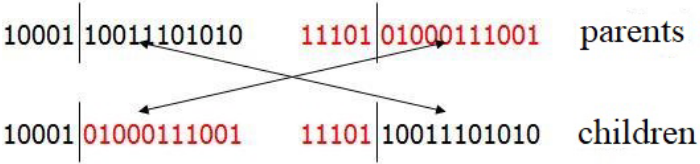
\includegraphics[width=0.65\columnwidth]{img/cross1}
	\end{center}
	Split both encodings in two and swap parts.\\
	
	\item \textbf{Double crossover:}
	\begin{itemize}
		\item extract two positions at random with uniform probability
		\item split the encoding in three parts at the extracted positions
		\item exchange the extreme parts of the encodings of the two individuals
	\end{itemize}
	\begin{center}
		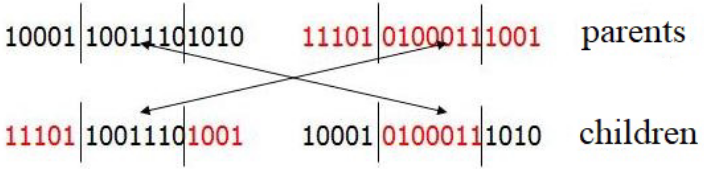
\includegraphics[width=0.65\columnwidth]{img/cross2}
	\end{center}
	Same as before but two "split positions".
\end{itemize}

\textbf{Generalizing}, one obtains the 
\begin{itemize}
	\item $\alpha$ \textbf{points crossover:}
	\begin{itemize}
		\item extract $\alpha$ positions at random with uniform probability
		\item split the encoding in $\alpha + 1$ parts at the extracted positions
		\item exchange the odd parts of the encodings of the two individuals (first, third, etc...)
	\end{itemize}
\end{itemize}

For small values of $\alpha$, this implies a \textbf{positional bias}: symbols \textbf{close in the encoding} tend to \textbf{remain close}. \\
To \textbf{cancel this bias}, one can adopt the
\begin{itemize}
	\item \textbf{Uniform crossover:}
	\begin{itemize}
		\item build a random binary vector $m \in U(\mathbb{B}^n)$ ("mask")
		\item if $m_i = 1$ exchange the symbols in position $i$ of the two individuals, if $m_i = 0$ keep them unmodified
	\end{itemize}
\end{itemize}

\newpage

\paragraph{Crossover versus Scatter Search and Path Relinking:} The crossover operator resembles the recombination phase of SS and PR.\\

The main differences are that
\begin{enumerate}
	\item It \textbf{recombines} the \textbf{symbols of the encodings}, instead of
	\begin{itemize}
		\item recombining the solutions (SS)
		\item performing a chain of exchanges on the solutions (PR)
	\end{itemize}
	\nn
	
	\item It \textbf{operates on the whole population}, instead of only a reference set $R$ (composed of only promising solution).\\
	
	\item It \textbf{operates on random pairs of individuals}, instead of methodically scanning all pairs of solutions in $R$.\\
	
	\item It \textbf{generates a pair of new individuals}, instead of
	\begin{itemize}
		\item generating a single intermediate solution (SS)
		\item visiting the intermediate solutions and choosing the best one (PR)
	\end{itemize}
	
	\item The \textbf{new individuals enter the population directly}, instead of becoming candidates for the reference set.\\
\end{enumerate}

However, classifying an operator can be a matter of taste.\\

\newpage

\subsubsection{Mutation}

The mutation operator \textbf{modifies an individual to generate a similar one}
\begin{itemize}
	\item scan encoding $\xi$ one symbol at a time
	\item decide with probability $\pi_m$ to modify the current symbol
\end{itemize}

The kind of modification usually depends on the encoding
\begin{itemize}
	\item \textbf{Binary encodings:} flip $\xi_i$ into $\xi_i' := 1 − \xi_i$ (changes value).\\
	
	\item \textbf{Symbol strings:} replace $\xi_c$ with a random symbol $\xi_c' \in B_c \setminus \{\xi_c \}$ selected with a uniform probability (change the symbol with another random possible one).\\
	
	\item \textbf{Permutations:} there are many proposals
	\begin{itemize}
		\item exchange two random elements in the permutation (swap)
		\item reverse the stretch between two random positions of the permutation
		\item ecc...
	\end{itemize}
	The symbols must remain all different from each other, otherwise it's not a permutation.\\
\end{itemize}

Basically, scan the encoding one symbol at a time and decide, with a certain probability, if mutating it, following one of the modifications described.\\

The mutation operator has strong relations with exchange operations.\\
The main differences are that
\begin{enumerate}
	\item it \textbf{modifies the symbols of an encoding}, instead of exchanging elements of a solution
	\item it \textbf{operates on random symbols}, instead of exploring a neighborhood systematically
	\item it \textbf{operates on a random subset of symbols of size unknown a priori}, somewhat like sampling a very large scale neighborhood, instead of exchanging a fixed number of elements
	\item it \textbf{operates on random individuals}, instead of all solutions
	\item the \textbf{new individuals enter the population directly}, instead of becoming candidates for the reference set
\end{enumerate}

\newpage

\subsubsection{The feasibility problem}
If the encoding is not fully invertible, \textbf{crossover and mutations sometimes generate encodings that do not correspond to feasible solutions}.\\

We distinguish between
\begin{itemize}
	\item \textbf{Feasible encodings} that \textbf{correspond} to \textbf{feasible solutions}.\\
	
	\item \textbf{Unfeasible encodings} that \textbf{correspond} to \textbf{legal, but unfeasible subsets}.\\
\end{itemize}

The \textbf{existence of unfeasible encodings} implies \textbf{several disadvantages}:
\begin{itemize}
	\item \textbf{inefficiency:} computational time is lost handling meaningless objects
	\item \textbf{ineffectiveness:} the heuristic explores fewer solutions (possibly, none)
	\item \textbf{design problems:} fitness must be defined also on unfeasible subsets
\end{itemize}
\nn

There are three main approaches to \textbf{face this problem}
\begin{enumerate}
	\item \textbf{Special encodings and operators:} (avoid or limit infeasibility).\\
	
	\item \textbf{Repair procedures:} (turn infeasibility into feasibility).\\
	
	\item \textbf{Penalty functions:} (accept infeasibility, but discourage it).\\
\end{enumerate}

\newpage

\paragraph{Special encodings and operators:} The idea is to investigate
\begin{itemize}
	\item \textbf{Encodings that} (nearly) \textbf{always yield feasible solutions}, such as
	\begin{itemize}
		\item permutation encodings and order-first split-second decodings for partition problems (CMSTP, VRP, etc...)
		\item permutation encodings and constructive heuristic decodings for scheduling problems (PMSP,...)
	\end{itemize}
	For example, if you use different symbols for each element and take an element from each alphabet you guarantee that the solution is a partition (if the problem is a partitioning problem).\\
	
	\item \textbf{Crossover and mutation operators that maintain feasibility}, such as
	\begin{itemize}
		\item operators that simulate moves on solutions ($k$-exchanges, for example for the TSP)
		\item specialized operators (Order or PMX crossover for the TSP)
	\end{itemize}
	If you start with a feasible solution, and thus a feasible encoding, if you only simulate moves that are part of the problem and keep the solution in the feasible space, the modified encoding will remain a feasible solution.\\
\end{itemize}

These methods
\begin{itemize}
	\item tend to closely \textbf{approximate exchange and recombination heuristics based on the concept of neighborhood}
	\item \textbf{give up the idea of abstraction} and \textbf{focus on the specific problem}, contrary to classical genetic algorithms
\end{itemize}
So, we're abandoning the idea of "general genetic algorithm" which work on encodings and don't care about the problem (really hard to put in practice, so kinda expected).\\

\newpage

\paragraph{Repair procedures:} A repair procedure is a \textbf{refined decoder function} $x_R : \, \Xi \rightarrow X$ that 
\begin{itemize}
	\item \textbf{decodes any encoding} $\xi$ into a \textbf{possibly unfeasible solution} $x (\xi) \notin X$
	\item \textbf{transforms} subset $x (\xi)$ \textbf{into a feasible solution} $x_R (\xi) \in X$
	\item returns $x_R$
\end{itemize}

The procedure is \textbf{applied to each unfeasible encoding} $\xi \in \Xi^{(g)}$
\begin{itemize}
	\item in some methods, \textbf{the encoding} $\xi (x_R (\xi))$ \textbf{replaces} $\xi$ \textbf{in} $X^{(g)}$ (you don't keep the encoding of the unfeasible solution, you manage only feasible solutions)
	\item in other ones, $\xi$ \textbf{remains in} $\Xi^{(g)}$ and $x_R (\xi)$ is \textbf{used only to update} $x^\ast$ (you keep the encoding of the unfeasible solutions, but use only the feasible one to update the best solution)
\end{itemize}

The methods of the first family
\begin{itemize}
	\item \textbf{maintain} a \textbf{population of feasible solutions}
\end{itemize}

but they introduce
\begin{itemize}
	\item a strong \textbf{bias in favor of feasible encodings}
	\item a \textbf{bias in favor of the feasible solutions most easily obtained} with the repair procedure
\end{itemize}

\newpage

\paragraph{Penalty functions:} Measuring the infeasibility, if the objective function is extended to unfeasible subsets $x \in 2^B \setminus X$, the fitness function $\phi (\xi)$ can be extended to any encoding, but \textbf{many unfeasible subsets have a fitness larger than the optimal solution}.\\

The selection operator tends to \textbf{favor such unfeasible subsets} (and the population becomes full of unfeasible subjects).\\

To avoid that, the \textbf{fitness function must combine}
\begin{itemize}
	\item the \textbf{objective value} $f (x (\xi))$
	\item a \textbf{measure of infeasibility} $\psi (x (\xi))$
	$$\begin{cases}
		\psi (x (\xi)) = 0 & \text{ if } x (\xi) \in X \\
		\psi (x (\xi)) > 0 & \text{ if } x (\xi) \notin X
	\end{cases}$$
	Basically, it's zero if it's feasible and it's positive if it's not, proportionally to how infeasible it is. How do we measure infeasibility?
\end{itemize}

If the constraints of the problem are expressed by equalities or inequalities, $\psi (x)$ can be defined as a weighted sum of their violations.\\
How to define the weights? Are they fixed, variable or adaptive?.\\

\newpage

\textbf{Definition} of the \textbf{fitness}: The most typical combinations are
\begin{itemize}
	\item \textbf{Absolute penalty:} minimize $\psi$ and $f$ lexicographically; given two encodings $\xi$ and $\xi'$ in a rank or tournament selection
	\begin{itemize}
		\item choose the less unfeasible one
		\item if they are equally (un)feasible, choose the better
	\end{itemize}
	Feasibility prevails on the cost, if one's feasible and one's not, always choose the first, otherwise choose the better/less unfeasible one.\\
	
	\item \textbf{Proportional penalty:} use a linear combination of $f$ and $\psi$
	$$ \varphi (\xi) = f (x (\xi)) - \alpha \psi (x (\xi)) + M \; \text{ for maximization problems} $$
	$$ \varphi (\xi) = -f (x (\xi)) - \alpha \psi (x (\xi)) + M \; \text{ for minimization problems} $$
	where offset $M$ guarantees that $\varphi (\xi) \geq 0$ for all encodings. The weight $\alpha$ tunes the importance of feasibility.\\
	
	\item \textbf{Penalty obtained by repair}, that is keep the unfeasible encoding, but derive its fitness from the objective value of the repaired solution
	$$ \varphi (\xi) = f (x_R (\xi)) \text{ or } \varphi (\xi) = UB - f (x_R (\xi)) $$
	since usually $f (x_R (\xi))$ is worse than $f (x (\xi))$ (unfeasible usually better than feasible). The objective function of the repaired solution is the fitness of the original one.\\
\end{itemize}

\newpage

\textbf{Weight tuning}: Experimentally, it is \textbf{better} to use the \textbf{smallest effective penalty}
\begin{itemize}
	\item If the penalty is \textbf{too small}, \textbf{too few feasible solutions} are \textbf{found}.\\
	
	\item If the penalty is \textbf{too large}, the \textbf{search is confined} within \textbf{a part of the feasible region} ("hidden" feasible solutions are hard to find).\\
\end{itemize}

A good value of the parameter $\alpha$ tuning the penalty can be found with
\begin{itemize}
	\item \textbf{Dynamic methods:} increase $\alpha$ over time according to a fixed scheme (first reach good subsets, then enforce feasibility).\\
	
	\item \textbf{Adaptive methods:} update $\alpha$ depending on the situation
	\begin{itemize}
		\item increase $\alpha$ when unfeasible encodings dominate the population (penalize unfeasibility more, go back to feasible solutions)
		\item decrease $\alpha$ when feasible encodings dominate (I want better solutions overall, care less about feasibility)
	\end{itemize}
	\nn
	
	\item \textbf{Evolutionary methods:} encode $\alpha$ in each individual (not only the current solution), in order to select and refine both the solution and the algorithm parameter. A vector inside the individual keeps the value of $\alpha$, to encode inside itself how it should move/evolve in the future.\\
\end{itemize}

\newpage

\subsection{Memetic algorithms}

Memetic algorithms (Moscato, 1989) are inspired by the concept of meme (Dawkins, 1976) that is a basic unit of reproducible cultural information
\begin{itemize}
	\item genes are selected only at the phenotypic expression level
	\item memes also adapt directly, as in Lamarckian evolution
\end{itemize}

Out of the metaphor, \textbf{memetic algorithms combine}
\begin{itemize}
	\item "\textbf{Genotypic}" operators that \textbf{manipulate the encodings} (crossover and mutation).\\
	
	\item "\textbf{Phenotypic}" operators that \textbf{manipulate the solutions} (local search).\\
\end{itemize}

In short, the \textbf{solutions are improved with exchanges before re-encoding}.\\

Several parameters determine how to apply local search
\begin{itemize}
	\item how often (at every generation, or after a sufficient diversification)
	\item to which individuals (all, the best ones, the most diversified ones)
	\item for how long (until a local optimum, beyond, or stopping before)
	\item with what method (steepest descent, VNS, ILS, etc...)
\end{itemize}

The idea is, you take some/all solutions encoded in the populations and improve them with exchanges, you have to decide how to apply exchange heuristics, how to apply the local search.\\
These are hybridized methods that take into account various other methods already described.\\

\newpage

\subsection{Evolution strategies}
They have been proposed by Rechenberg and Schwefel (1971).\\

The main differences with respect to classical genetic algorithms are:
\begin{itemize}
	\item The \textbf{solutions} are \textbf{encoded} into \textbf{real vectors}.\\
	
	\item A \textbf{small population of} $\mu$ \textbf{individuals generate} $\lambda$ \textbf{candidate descendants} (originally, $\mu = 1$).\\
	
	\item The \textbf{new individuals compete to build the new population}
	\begin{itemize}
		\item in the $(\mu, \lambda)$ strategy the best $\mu$ descendants replace the original population, even if some are dominated
		\item in the $(\mu + \lambda)$ strategy the best $\mu$ individuals overall (predecessors or descendants) survive in the new population
	\end{itemize}
	\nn
	
	\item The \textbf{mutation} operator \textbf{sums to the encoding a random noise with a normal distribution of zero average}
	$$ \xi' := \xi + \delta \text{ with } \delta \in N(0, \sigma) $$
	basically a disturbance taken from a distribution.\\
	
	\item Originally, the crossover operator was not used (now it is)
\end{itemize}

The random-key genetic algorithm (Bean, 1994) use real-vector encodings and decode procedures based on sorting the real numbers.\\

% End of L23, last lesson is lab, so it ends here, farewell space cowboy